%%% LaTeX Template: Article/Thesis/etc. with colored headings and special fonts
%%%
%%% Source: http://www.howtotex.com/

\documentclass[12pt]{article}


\usepackage{apuntes-estilo}
\usepackage{fancyhdr,lastpage}
\usepackage{color,colortbl}
\usepackage{verbatim}

\def\maketitle{

% Titulo 
 \makeatletter
 {\color{bl} \centering \huge \sc \textbf{
 Manteniendo la hora \\ 
\large \vspace*{-8pt} \color{black} Guía básica de mantenimiento de la hora
 \vspace*{8pt} }\par}
 \makeatother


% Autor
 \makeatletter
 {\centering \small 
 	Departamento de Ingeniería de Computadoras \\
 	Facultad de Informática - Universidad Nacional del Comahue \\
 	\vspace{20pt} }
 \makeatother

}

% Custom headers and footers
\fancyhf{} % clear all header and footer fields
\fancypagestyle{plain}{\fancyhf{}}
  	\pagestyle{fancy}
 	\lhead{\footnotesize Manteniendo la hora - Departamento de Ingeniería de Computadoras}
 	\rhead{\footnotesize \thepage\ }	% ''Page 1 of 2''

\def\ti#1#2{\texttt{#1} & #2 \\ }



\begin{document}

\thispagestyle{empty}
\maketitle
\setlength{\parindent}{0pt}

\section*{ Manteniendo La Hora}

En este capítulo se explica como un sistema Linux mantiene la fecha y hora,
y lo que debe conocer para evitar problemas. Si bien el mantenimiento de
la hora no es una actividad frecuente, es resposabilidad del administrador 
del sistema realizar los cambios que sean necearios. 


\subsection*{Zonas horarias}

Las mediciones horarias están basadas en su mayoría a fenómenos naturales regulares,
como por ejemplo, los periodos alternados de luz y oscuridad
causados por la rotación del planeta. El tiempo total tomado por dos períodos
sucesivos es constante, pero la duración del período de luz varía
con respecto al de oscuridad. Una constante simple es la luz del mediodía.

El mediodía es el momento del día en el cual el Sol se encuentra en la posición más alta. 
Debido a la rotación de la Tierra, el momento del mediodía sucede en diferentes 
momentos en diferentes lugares. Esto nos conduce al concepto de \textit{hora local}.
Si permanecemos siempre en el mismo lugar, las diferencias entre los
horarios locales de diferentes sitios pareciera no tienen mucha importancia.

Sin embargo, en cuanto necesite comunicarse con lugares distantes, con horarios locales 
diferentes, notará la necesidad de una hora en común. Hoy en día, la mayoría de los lugares en el mundo deben
comunicarse con otros, por lo que se definió un estándar mundial de medición
horaria. Este estándar se llama \textit{hora universal} ó UTC (del inglés Universal 
Time Coordinated), y es uno de los varios sucesores estrechamente 
relacionados con el tiempo medio de Greenwich (GMT). De hecho, aunque técnicamente 
difieren GMT y UTC suelen utilizarce como sinónimos en mucha bibliografía.   
De este modo, cuando personas con diferentes horas locales
necesitan comunicarse, pueden expresar el tiempo en hora universal,
para que no exista confusión acerca de cuándo deben suceder las cosas.

Cada hora local es llamada zona horaria (time zone), y existen 24 zonas horarias
en el planeta. Si bien geográficamente es posible pensar que todos los lugares
en donde el mediodía suceda en el mismo momento tienen la misma zona horaria,
políticamente esto no siempre así. Por diversas razones, varios países
adoptan el ``horario de verano'' (\textit{daylight savings time} o DST) para atender las demandas
económicas. Los países que adoptan el ``horario de verano'' cambian la hora
de sus relojes en verano (en gral. se retrasan los relojes una hora) para
tener más luz natural mientras trabajan (durante la tarde), y vuelven a adelantar
la hora de sus relojes en otoño o invierno. Otros países no adoptan estos procedimientos.
Más aún, los países que utilizan horarios de verano no tienen un acuerdo común de cuándo deben
modificarse los relojes, y cambian, además, las reglas año tras año. Por lo que las
conversiones de zonas horarias son definitivamente no-triviales.

\begin{center}
 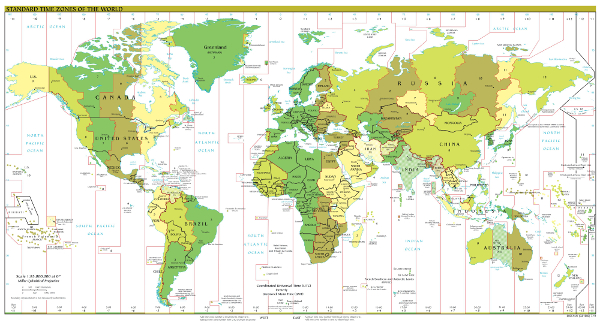
\includegraphics{World_Time_Zones_Map.jpg}
\end{center}

Las zonas horarias son denominadas de mejor manera a través de su ubicación o por
la diferencia entre la hora universal y la hora local. En la Argentina y
en algunos otros países, las zonas horarias locales tienen un nombre y una abreviatura
de tres letras (ART en nuestro caso). Las abreviaturas \textbf{no son únicas}, por lo que no deberían
ser utilizadas sin que aparezca también el nombre del país. Es mejor referirse a la
la hora local en Helsinki, que referirse a la hora del Este de Europa, debido a que
no todos los países del Este de Europa adoptan las mismas reglas. De hecho dentro 
de nuestro país, Argentina,  ha sucedido que diferentes provincias utilicen diferentes
zonas horarias. \footnote{Ver http://es.wikipedia.org/wiki/Hora\_oficial\_argentina}


GNU/Linux tiene un paquete de zonas horarias que reconoce todas las zonas horarias existentes,
y puede ser fácilmente actualizado cuando las reglas cambian. Todo lo que un administrador de 
sistemas necesita hacer es seleccionar la zona horaria apropiada. A su vez, cada usuario 
puede establecer su propia zona horaria (recordemos que GNU/Linux es un sistema multiusuario); 
por lo que facilita el trabajo de mucha gente, debido a que muchas personas trabajan en diferentes 
países a través de Internet y quizá sobre el mismo equipo.
Cuando las reglas del ``horario de verano'' cambian para el horario local de los equipos que 
administra, asegúrese de actualizar al menos la zona horaria del sistema y de ser necesario 
la definición de zonas horarias disponibles. 


\subsection*{ Los relojes de software y hardware}


En general las computadoras tiene un reloj de hardware alimentado por una batería, conocido también como 
``reloj de tiempo real'' o RTC (del inglés \textit{Real Time Clock}). 
Esa batería asegura que el reloj continúe trabajando aún cuando la computadora se encuentre sin
suministro eléctrico. El reloj de hardware puede ser modificado (o definido)
desde el firmware inicial que controla la placa base, como por ejemplo el BIOS en las 
computadoras personales, o desde cualquier sistema operativo.

Por otra parte, una vez iniciado el sistema, el kernel Linux mantiene la fecha y hora 
de manera independiente al reloj de hardware. Este reloj es conocido como ``reloj de sistema'', 
``reloj de software'' o ``reloj del kernel''. 
Durante el inicio de un sistema Linux, el kernel configura su propio reloj de software accediendo
a la fecha y hora mantenida por el reloj de hardware.
Luego, ambos relojes trabajan independientemente.
Linux mantiene su propio reloj debido a que leer el reloj de hardware constantemente es 
lento, complicado e inexacto.

El reloj del kernel siempre muestra la hora universal, por lo que
no necesita conocer como utilizar husos horarios. La simplicidad de este
modo de trabajar proporciona alta confiabilidad y facilita actualizar 
la información de la zona horaria. Cada proceso realiza las conversiones de zona horaria 
de manera independiente (utilizando herramientas estándar que son parte del paquete de zona horaria).


El reloj de hardware puede estar en formato de hora local u hora universal.
Usualmente es mejor que el reloj de hardware mantenga la hora universal,
porque de esta manera no será necesario modificar la hora del reloj cuando el ``horario de verano''
(daylight savings time o DST) empiece o finalice (UTC no tiene DST). Desafortunadamente, algunos sistemas operativos 
(por ejemplo MS-DOS, Windows y OS/2) asumen que el reloj de hardware muestra la hora local.
Por otra parte, Linux puede manejar cualquiera de los dos formatos, pero si el reloj de hardware muestra la hora local,
entonces debe modificarlo cada vez que el ``horario de verano'' empiece o finalice. Este 
punto es particularmente conflictivo en equipos donde coexisten más de un 
sistema operativo (clásico dual boot Windows-GNU/Linux). 


\subsection*{Configurar y visualizar la hora}

En Linux, la zona horaria del sistema es determinada por \texttt{/etc/localtime} (algunas veces
es un enlace simbólico). Si es un enlace, entonces apunta a un archivo de datos de zona horaria
que describe la zona horaria local. Los archivos de datos de zonas horarias están ubicados en
\texttt{/usr/lib/zoneinfo} o \texttt{/usr/share/zoneinfo}. (Esto puede variar según la 
distribución particular de GNU/Linux utilizada). 

Por ejemplo, en un sistema SuSE ubicado en Santiago de Chile \texttt{/etc/localtime} apuntaría
a \texttt{/usr/share/zoneinfo/Chile/Continental (UTC-4)}.

Si no encuentra el directorio \texttt{zoneinfo} en \texttt{/usr/lib} o en \texttt{/usr/share}, 
intente encontrarlo ejecutando \texttt{\textbf{find /usr -type d -name zoneinfo}}, o consulte 
la documentación de su distribución GNU/Linux particular.

\textbf{Múltiples usuarios en diferentes zonas horarias:}

¿Qué sucede cuando existen usuarios utilizando el mismo sistema pero se encuentran ubicados en
zonas horarias diferentes?
Un usuario puede cambiar su zona horaria privada definiendo la variable de ambiente TZ.
Si TZ no se encuentra definida, entonces la zona horaria del sistema es la utilizada.
La sintaxis de la variable TZ se encuentra descripta en la página de manual de \texttt{\textbf{tzset}}.


\colorbox{grey}{\parbox[t]{0.95\linewidth}{ \vspace*{0.5cm} { 
Por ejemplo si la hora local del sistema esta definida para Argentina, tal que 
el comando \texttt{date} nos devuelve: \\
{\tt\$ date \\
mié jul 31 17:14:40 ART 2013} \\
Y ahora definimos la variable de ambiente TZ con el valor (Eastern Standard Time, utilizada en 
algunas regiones de Estados Unidos), veremos que la salida de \texttt{date} responde 
a la nueva hora local utilizada por el usuario: \\
{\tt
\$ export TZ=EST \\
\$ date \\
mié jul 31 15:14:53 EST 2013 \\
} 
Esto es, dos horas de diferencia con la hora local Argentina. 
 } \vspace*{0.5cm} } } 


El comando \texttt{\textbf{date}} muestra la hora y fecha actuales. Por ejemplo:



\colorbox{grey}{\parbox[t]{0.95\linewidth}{ \vspace*{0.5cm} {\tt 
\$ date \\
mié jul 31 17:14:40 ART 2013
 } \vspace*{0.5cm} } } 

Es decir, miércoles 31 de julio del 2013, cinco y cuarto de la tarde en hora local Argentina  \textit{``ART''}.
El comando \texttt{\textbf{date}} también puede también mostrar la hora universal (UTC): 



\colorbox{grey}{\parbox[t]{0.95\linewidth}{ \vspace*{0.5cm} {\tt 
\$date -u\\
mié jul 31 20:18:02 UTC 2013
 } \vspace*{0.5cm} } } 


\texttt{\textbf{date}} también se utiliza para establecer la hora del reloj del kernel. Para más información
lea la página de manual de \texttt{\textbf{date}}. Tenga en cuenta que \textbf{solo el usuario root puede 
modificar la fecha y/u hora del sistema}. Aunque cada usuario puede definir su propia zona horaria, el reloj 
es el mismo para todos.

\texttt{\textbf{date}} muestra o modifica el reloj de software. El comando \texttt{\textbf{hwclock}} 
sincroniza los relojes de hardware y software.
Cuando el sistema inicia, el comando \texttt{hwclock} es utilizado para leer el reloj de hardware y actualizar
el reloj de software. Si necesita modificar ambos relojes, primero debe modificar el reloj de software con \texttt{\textbf{date}},
y luego sincronizar la hora del reloj por hardware con el comando \texttt{\textbf{hwclock -w o hwclock --systohc}}.

La opción \texttt{ ``-u o --utc''} en el comando \texttt{\textbf{hwclock}} le indica 
a \texttt{hwclock} que la fecha y hora (mostrada o definida)
se encuentra en formato de hora universal. \textit{Debe} utilizar la opción -u correctamente, en
caso contrario, la computadora puede estar confundida sobre cual es la fecha y hora correcta.



Los relojes deben modificarse con cuidado y precisión.
Muchas partes de un sistema UNIX requieren que los relojes trabajen correctamente.
Por ejemplo, el demonio \texttt{\textbf{cron}} ejecuta comandos periódicamente. Si cambia el reloj, el sistema puede
estar confundido en cuanto a la necesidad o no de ejecutar determinado comando.
Hubo una vez, en un sistema UNIX antiguo, en donde alguien adelantó el reloj 20 años en el futuro, y
entonces \texttt{\textbf{cron}} quiso ejecutar
los comandos periódicos de veinte años, todos de una sola vez.
Las versiones actuales de \texttt{\textbf{cron}} no tienen este problema, pero aún así debe ser cuidadoso con estos
detalles (pueden existir otros programas actuales que trabajen similarmente mal como ``ese'' viejo cron).
Grandes saltos en el tiempo (hacia el futuro o el pasado) son mas peligrosos que pequeñas diferencias.




\section*{Cuando el reloj es erróneo}


El reloj por software de un sistema Linux no siempre es preciso. Para mantener este reloj
Linux utiliza una \textit{interrupción periódica} generada por el hardware, llamada ``timer interrupt''.
En caso de que existan muchos procesos siendo ejecutados (con respecto a los recursos disponibles)
el sistema podría demorar un poco al momento de intentar servir la interrupción, por lo que 
el reloj de software puede estar ligeramente atrasado. El reloj por hardware trabaja
independientemente del sistema operativo, así que usualmente es mas preciso. 
Si re-inicia de manera frecuente la computadora (como es el caso para la mayoría de los
sistemas que no son servidores) el reloj debe encontrarse prácticamente correcto.



Si es necesario modificar el reloj de hardware, la manera mas simple es reiniciar el sistema,
ingresar a la pantalla de configuración de la BIOS y realizar el cambio de fecha y hora desde
ahí. Esta manera evita todos los problemas que podrían suceder si se modifica el reloj desde 
el sistema. Si la modificación desde la configuración de la BIOS no se puede realizar, modifique
el reloj utilizando \texttt{\textbf{date}} y \texttt{\textbf{hwclock}} (en ese orden), pero 
esté preparado para reiniciar Linux, si alguna parte del sistema comienza a actuar de manera 
extraña, mal y/o divertida. :)



Otro método posible para sincronizar el reloj de software es utilizar \texttt{\textbf{hwclock -w}} o \texttt{\textbf{hwclock --systohc}}.
Ambos comandos obtienen la fecha y hora desde el reloj de hardware y modifican el reloj de software.
Si en cambio desea sincronizar de manera inversa (modificar el reloj de hardware con la fecha y
hora del reloj de software) entonces puede utilizar el comando \texttt{\textbf{hwclock -s}} o el comando
\texttt{\textbf{hwclock --hctosys}}. Si desea conocer mayores detalles de este comando lea su página de manual
ejecutando man \texttt{\textbf{hwclock}}.


\section*{NTP - Protocolo de reloj en red}


Un ordenador conectado en red (incluso únicamente con un módem) puede 
comprobar su propio reloj de forma automática comparándolo con la hora
de otro ordenador que se sabe almacena la hora de forma precisa. El 
protocolo de reloj en red (o NTP) hace esto exactamente. Es un método para 
verificar y corregir la hora de su ordenador al sincronizarse con otro 
sistema. Con NTP su sistema puede mantenerse a milisegundos de la Hora 
Universal Coordinada. 
	\footnote{Visite el sitio web <ulink url=``http://www.time.gov/about.html/''>
		http://www.time.gov/about.html</ulink> si desea obtener mayor información.
		}
	


Para la mayoría de usuarios ocasionales de Linux, esto puede resultar
simplemente un lujo. En mi casa todos los relojes se ajustan en base a 
la hora que mi sistema Linux dice que es. Para grandes organizaciones 
este ``lujo'' puede convertirse en fundamental. Ser capaz de buscar sucesos 
en los archivos de diario basándose en la hora puede hacer la vida 
bastante más sencilla y puede eliminar mucho ``trabajo de adivinación'' 
durante la depuración.



Otro ejemplo de cuan importante puede ser NTP es con SAN. Algunos SAN
necesitan NTP para configurarse y funcionar adecuadamente para permitir
la correcta sincronización durante el uso del sistema de ficheros, y un
control adecuado de las marcas de tiempo. Algunos SAN (y algunas
aplicaciones) pueden confundirse cuando tratan con archivos que tienen marcas
de tiempo que están en el futuro.



La mayoría de las distribuciones Linux vienen con un paquete NTP de
algún tipo, ya sea un paquete .deb o .rpm. Puede utilizarlo para instalar
NTP, o puede bajarse el código fuente de
<ulink url=``http://www.ntp.org/downloads.html''>
http://www.ntp.org/downloads.html</ulink> y compilarlo usted mismo. En
cualquier caso, la configuración básica es la misma.





\section*{ Configuración básica de NTP}


El programa NTP se configura utilizando el archivo \texttt{/etc/ntp.conf} o
\texttt{/etc/xntp.conf} dependiendo de qué distribución Linux tenga. No entraré
ahora en demasiados detalles sobre cómo configurar NTP. En su lugar cubriré
sólo lo básico.



Un ejemplo de archivo ntp.conf debería parecer:



\colorbox{grey}{\parbox[t]{0.95\linewidth}{ \vspace*{0.5cm} {\tt
\# --- GENERAL CONFIGURATION ---
server  aaa.bbb.ccc.ddd
server  127.127.1.0
fudge   127.127.1.0 stratum 10

\# Drift file.
driftfile /etc/ntp/drift
 } \vspace*{0.5cm} } } 

	

	El archivo ntp.config más básico simplemente listará 2 servidores, uno
con el que le gustaría sincronizarse, y una dirección pseudo-IP para él 
mismo (en este caso 127.127.1.0). La pseudo-IP se utiliza en el caso de
errores en la red o si cae el servidor NTP remoto. NTP sincronizará
consigo mismo hasta que pueda empezar a sincronizar de nuevo con el 
servidor remoto. Se recomienda que se pongan al menos 2 servidores remotos
con los que pueda sincronizarse. Uno actuará como servidor primario y el 
otro como copia de respaldo.



También debe ponerse una ubicación para el archivo de fluctuación. De 
vez en cuando NTP \textit{aprenderá} el error que se comete en el reloj de
sistema y automáticamente se ajustará.



La opción de restricción puede usarse para otorgar un mejor control y 
seguridad además de la que proporciona NTP, y quién puede efectuarla.
Por ejemplo:

\colorbox{grey}{\parbox[t]{0.95\linewidth}{ \vspace*{0.5cm} {\tt 
\#Prohibit general access to this service.
restrict default ignore

\# Permit systems on this network to synchronize with this
\# time service. But not modify our time.
restrict aaa.bbb.ccc.ddd nomodify

\# Allow the following unrestricted access to ntpd

restrict aaa.bbb.ccc.ddd
restrict 127.0.0.1
 } \vspace*{0.5cm} } } 


Está avisado: debe esperar hasta que tenga NTP trabajando adecuadamente 
antes de añadir la opción de restricción. Puede accidentalmente 
restringirse usted mismo de sincronizarse y perder tiempo buscando el por qué.



NTP corrige el sistema lentamente. ¡Sea paciente! Una simple prueba es
cambiar el reloj de sistema en 10 minutos antes de irse a la cama y
comprobarlo cuando se levante. La hora deberá ser la correcta.

\section*{ La herramienta NTP}


Hay innumerables utilidades disponibles para comprobar si NTP está 
haciendo su trabajo. El comando \texttt{\textbf{ntpq -p}} mostrará el estado de la hora
actual de su sistema.


\colorbox{grey}{\parbox[t]{0.95\linewidth}{ \vspace*{0.5cm} {\tt      
ntpq -p
remote           refid      st t when poll reach   delay   offset  jitter
==============================================================================
*cudns.cit.corne ntp0.usno.navy.  2 u  832 1024  377   43.208    0.361   2.646
 LOCAL(0)        LOCAL(0)        10 l   13   64  377    0.000    0.000   0.008
 } \vspace*{0.5cm} } } 

	
\texttt{\textbf{ntpdc -c}} loopinfo mostrará cómo de desviado está el reloj del sistema
en segundos, basándose en la última vez que se contactó con el servidor 
remoto.



\colorbox{grey}{\parbox[t]{0.95\linewidth}{ \vspace*{0.5cm} {\tt 
ntpdc -c loopinfo
offset:               -0.004479 s
frequency:            133.625 ppm
poll adjust:          30
watchdog timer:       404 s
 } \vspace*{0.5cm} } } 

	
\texttt{\textbf{ntpdc -c kerninfo}}  mostrará la corrección actual acumulada.


\colorbox{grey}{\parbox[t]{0.95\linewidth}{ \vspace*{0.5cm} {\tt 
ntpdc -c kerninfo
pll offset:           -0.003917 s
pll frequency:        133.625 ppm
maximum error:        0.391414 s
estimated error:      0.003676 s
status:               0001  pll
pll time constant:    6
precision:            1e-06 s
frequency tolerance:  512 ppm
pps frequency:        0.000 ppm
pps stability:        512.000 ppm
pps jitter:           0.0002 s
calibration interval: 4 s
calibration cycles:   0
jitter exceeded:      0
stability exceeded:   0
calibration errors:   0
 } \vspace*{0.5cm} } } 

	
Una versión ligeramente distinta de \texttt{\textbf{ntpdc -c kerninfo}} es \texttt{\textbf{ntptime}}


\colorbox{grey}{\parbox[t]{0.95\linewidth}{ \vspace*{0.5cm} {\tt 
ntptime
ntp\_gettime() returns code 0 (OK)
  time c35e2cc7.879ba000  Thu, Nov 13 2003 11:16:07.529, (.529718),
  maximum error 425206 us, estimated error 3676 us
ntp\_adjtime() returns code 0 (OK)
  modes 0x0 (),
  offset -3854.000 us, frequency 133.625 ppm, interval 4 s,
  maximum error 425206 us, estimated error 3676 us,
  status 0x1 (PLL),
  time constant 6, precision 1.000 us, tolerance 512 ppm,
  pps frequency 0.000 ppm, stability 512.000 ppm, jitter 200.000 us,
  intervals 0, jitter exceeded 0, stability exceeded 0, errors 0.
 } \vspace*{0.5cm} } } 

	
	
	

Existe todavía otra manera de ver cómo de bien está trabajando NTP con 
el comando \texttt{\textbf{ntpdate -d}}. Éste contactará con un servidor NTP y
determinará la diferencia de tiempos pero no modificará el reloj de su sistema.



\colorbox{grey}{\parbox[t]{0.95\linewidth}{ \vspace*{0.5cm} {\tt 
ntpdate -d 132.236.56.250
13 Nov 14:43:17 ntpdate[29631]: ntpdate 4.1.1c-rc1@1.836 Thu Feb 13 12:17:20 EST 2003 (1)
transmit(132.236.56.250)
receive(132.236.56.250)
transmit(132.236.56.250)
receive(132.236.56.250)
transmit(132.236.56.250)
receive(132.236.56.250)
transmit(132.236.56.250)
receive(132.236.56.250)
transmit(132.236.56.250)
server 132.236.56.250, port 123
stratum 2, precision -17, leap 00, trust 000
refid [192.5.41.209], delay 0.06372, dispersion 0.00044
transmitted 4, in filter 4
reference time:    c35e5998.4a46cfc8  Thu, Nov 13 2003 14:27:20.290
originate timestamp: c35e5d55.d69a6f82  Thu, Nov 13 2003 14:43:17.838
transmit timestamp:  c35e5d55.d16fc9bc  Thu, Nov 13 2003 14:43:17.818
filter delay:  0.06522  0.06372  0.06442  0.06442
         0.00000  0.00000  0.00000  0.00000
filter offset: 0.000036 0.001020 0.000527 0.000684
         0.000000 0.000000 0.000000 0.000000
delay 0.06372, dispersion 0.00044
offset 0.001020

13 Nov 14:43:17 ntpdate[29631]: adjust time server 132.236.56.250 offset 0.001020 sec
 } \vspace*{0.5cm} } } 

Si quiere ver al sistema sincronizarse en tiempo real puede utilizar 
\texttt{\textbf{ntptrace}}.


\colorbox{grey}{\parbox[t]{0.95\linewidth}{ \vspace*{0.5cm} {\tt 
ntptrace 132.236.56.250
cudns.cit.cornell.edu: stratum 2, offset -0.003278, synch distance 0.02779
dtc-truetime.ntp.aol.com: stratum 1, offset -0.014363, synch distance 0.00000, refid 'ACTS' 
} \vspace*{0.5cm} } } 

	

	
	
Si necesita sincronizar su sistema inmediatamente puede utilizar
\texttt{\textbf{ntpdate remote-servername}} para forzar una sincronización. ¡Sin esperas!


\colorbox{grey}{\parbox[t]{0.95\linewidth}{ \vspace*{0.5cm} {\tt
ntpdate 132.236.56.250
13 Nov 14:56:28 ntpdate[29676]: adjust time server 132.236.56.250 offset -0.003151 sec
  } \vspace*{0.5cm} } } 


\section*{ Algunos servidores NTP conocidos}


Una lista de servidores públicos puede obtenerse de:
<ulink url=``http://www.eecis.udel.edu/~mills/ntp/servers.html/''>
	http://www.eecis.udel.edu/~mills/ntp/servers.html</ulink>. Por favor lea la
información de utilización de la página antes de utilizar un servidor. No 
todos los servidores tienen el suficiente ancho de banda para permitir 
un gran número de sistemas sincronizándose con ellos. Así que es buena 
idea contactar con el administrador de sistemas antes de utilizar su 
servicio NTP.



\section*{ Enlaces NTP}


Información más detallada sobre NTP puede obtenerse de la página
original NTP: <ulink url=``http://www.ntp.org/''>http://www.ntp.org</ulink>, o de
<ulink url=``http://www.ntp.org/ntpfaq/NTP-a-faq.htm''>
	http://www.ntp.org/ntpfaq/NTP-a-faq.htm</ulink>


\section*{Licencia}

Este material es una obra derivada de los siguientes textos:

http://tldp.org/HOWTO/Clock.html\#toc2

``Sistema operativo GNU/Linux Básico'' \footnote{http://materials.cv.uoc.edu/continguts/XW07\_M2102\_02309/index.html}

© Autores: Joaquín López Sánchez-Montañés, Sofia Belles Ramos, Roger Baig i Viñas i Francesc Aulí Llinàs

© 2008, FUOC. Se garantiza permiso para copiar, distribuir y modificar este documento según los
términos de la GNU Free Documentation License, Version 1.2 o cualquiera posterior publicada por la
Free Software Foundation, sin secciones invariantes ni textos de cubierta delantera o trasera. Se dispone
de una copia de la licencia en el apartado ``GNU Free Documentation License'' de este documento.

\begin{thebibliography}{1}
\bibitem[CurLinux]{curlin} ``Curso de Linux''.1999 Gómez, Ahijado, Flores.\\ 
http://www.ibiblio.org/pub/Linux/docs/LuCaS/Tutoriales/CURSOLINUX/\\curso\_linux/curso\_linux.html
\end{thebibliography}

\end{document}
